\documentclass[11pt]{article}

\usepackage[utf8]{inputenc}
\usepackage[T1]{fontenc}
\usepackage[provide=*,spanish]{babel}
\usepackage[a4paper,margin=2.4cm]{geometry}
\usepackage{amsmath,amssymb}
\usepackage{booktabs}
\usepackage{graphicx}
\usepackage{float}
\usepackage{enumitem}
\usepackage[expansion=false]{microtype}
\usepackage{xcolor}
\usepackage[hidelinks]{hyperref}

\graphicspath{{figs/}}
\newcommand{\Roos}{$R^2_{\text{oos}}$}

\title{\vspace{-1.2cm}\textbf{Optimización de portafolio en el IPSA:\\
¿Una estrategia sofisticada le gana al 1/N?}}

\author{Carlos Tapia \quad Mauricio Pizarro \quad Brian Valenzuela\\[2pt]
\small INF398 --- Introducción al Aprendizaje Automático}

\begin{document}
\maketitle
\vspace{-0.6cm}

\section{Objetivo y enfoque}
Construimos estrategias de inversión relativamente sofisticadas para un portafolio de acciones del
IPSA y las pusimos a prueba contra dos referencias simples. La pregunta no es sólo cuál rinde más,
sino si las diferencias observadas son \textbf{estadísticamente robustas o apenas ruido} del período
analizado. El objetivo no es demostrar que el \emph{Machine Learning} (ML) gana: si no mejora al
benchmark, ese resultado es igual de válido y lo reportamos como tal.

Exploramos dos familias de modelos ML. La primera \textbf{predice el retorno esperado} $\mu$ de cada
acción y entrega ese vector a un optimizador de cartera (Ridge, Lasso, Elastic Net y un MLP). La
segunda es un \textbf{MLP de asignación directa} (\emph{decision-focused learning}, DFL): en lugar de
predecir retornos, la red produce directamente los pesos del portafolio, entrenada para maximizar el
Sharpe. La idea de esta segunda familia es saltarse el paso intermedio de predecir $\mu$ y optimizar
la métrica que realmente importa.

Sobre esa base, la estrategia combina cinco ingredientes:
\begin{itemize}[nosep,leftmargin=*]
  \item \textbf{Predicción de retornos con ML}, con la regularización elegida sin mirar el futuro.
  \item \textbf{Covarianza robusta} mediante \emph{shrinkage} de Ledoit--Wolf, que estabiliza la
  matriz de riesgo cuando hay pocos datos.
  \item \textbf{Validación walk-forward}: en cada mes se estiman los parámetros con datos pasados y se
  aplican al mes siguiente, sin acceso a información futura.
  \item \textbf{Costos de transacción} de $0.1\%$ por rebalanceo.
  \item \textbf{Restricciones de concentración}: pesos acotados por acción, para no depender de una
  sola apuesta.
\end{itemize}

Las comparamos contra dos benchmarks: el reparto ingenuo 1/N (pesos iguales) y el Markowitz histórico
de máximo Sharpe. Adelantamos el resultado central: \textbf{algunas métricas mejoran marginalmente
sobre el 1/N, pero esas mejoras no resisten un test de significancia}, y el 1/N permanece
extremadamente competitivo.

\section{Datos y metodología}
\label{sec:metodologia}

\paragraph{Universo y datos.} Trabajamos con 21 acciones del IPSA con historia disponible desde 2008,
sobre retornos mensuales. Los precios de cierre ajustados se descargan una vez de Yahoo Finance y se congelan en un CSV, de modo que los resultados aquí reportados son reproducibles entre corridas. Se descartan
acciones con demasiados datos faltantes y se recortan retornos extremos ($\pm 40\%$ mensual) para
tratar \emph{outliers}. Se obtienen 203 meses de retornos (feb.~2008--dic.~2024).

\paragraph{Features sin mirar el futuro.} Para cada acción construimos 9 \emph{features} a partir de
sus propios retornos (momentum a 1/3/6/12 meses, volatilidad a 3 y 6 meses, media móvil, desviación
respecto de esa media y un RSI). Todas van rezagadas un mes: en el mes $t$ sólo se usa información
disponible hasta $t-1$, y el objetivo a predecir es el retorno de $t$. La matriz final es de $191$
meses $\times\, 189$ columnas (9 por acción). La evaluación es \textbf{walk-forward}: en cada mes se
estiman los parámetros con los $36$ meses previos y se aplican al mes siguiente. Así el modelo nunca
ve el dato que intenta predecir, siendo una forma honesta de medir su desempeño. El período de
test resultante es de \textbf{155 meses} (feb.~2012--dic.~2024).

\paragraph{Las seis estrategias.} Comparamos: (1) el reparto ingenuo 1/N; (2) Markowitz clásico
($\mu$ histórico y covarianza muestral); (3) Markowitz con covarianza Ledoit--Wolf; (4) mínima
varianza con Ledoit--Wolf, que \emph{no} usa retornos esperados; (5) el ML Ridge, que predice $\mu$ y
lo entrega al optimizador de máximo Sharpe; y (6) el DFL, el MLP que asigna pesos directamente. En
todos los casos que optimizan, la covarianza se estabiliza con \emph{shrinkage} de Ledoit--Wolf y los
pesos se obtienen resolviendo un problema convexo (\texttt{cvxpy}) con suma $1$ y cotas por acción
$[0,\,0.20]$. Se descuentan costos de $0.1\%$ por rebalanceo.

\paragraph{Cómo elegimos los hiperparámetros: MSE vs.\ Sharpe.} En la línea base, los modelos que
predicen $\mu$ eligen su regularización minimizando el error de predicción (MSE), acción por acción.
Como variante, probamos elegirla optimizando directamente el \textbf{Sharpe} de la cartera sobre un
tramo de validación interno a la ventana (los últimos 12 meses), sin tocar nunca el período de test.
Esto responde una duda natural: ¿y si afinamos el modelo para la métrica que de verdad nos importa,
en vez del error de predicción? La respuesta, adelantamos, es que no ayuda.

\paragraph{Test de significancia.} Para decidir si las diferencias de Sharpe son reales o ruido,
usamos un \emph{bootstrap} por bloques sobre los retornos fuera de muestra (5000 réplicas, bloques de
6 meses, remuestreo pareado). De ahí obtenemos, para cada estrategia, el intervalo de confianza al
95\% de su Sharpe y el $p$-valor de la diferencia contra el 1/N.

\section{Resultados}
\label{sec:resultados}

La Figura~\ref{fig:eda} resume el universo: precios normalizados, retorno mensual promedio,
volatilidad anualizada por acción y matriz de correlaciones. Destaca la fuerte dispersión de
volatilidades, desde niveles en torno al $22\%$ en las acciones más defensivas hasta sobre $40\%$ en
las mineras (CAP, SQM-B), y las correlaciones mayormente moderadas, salvo pares ligados por control
común, como Copec--AntarChile.

\begin{figure}[H]
\centering
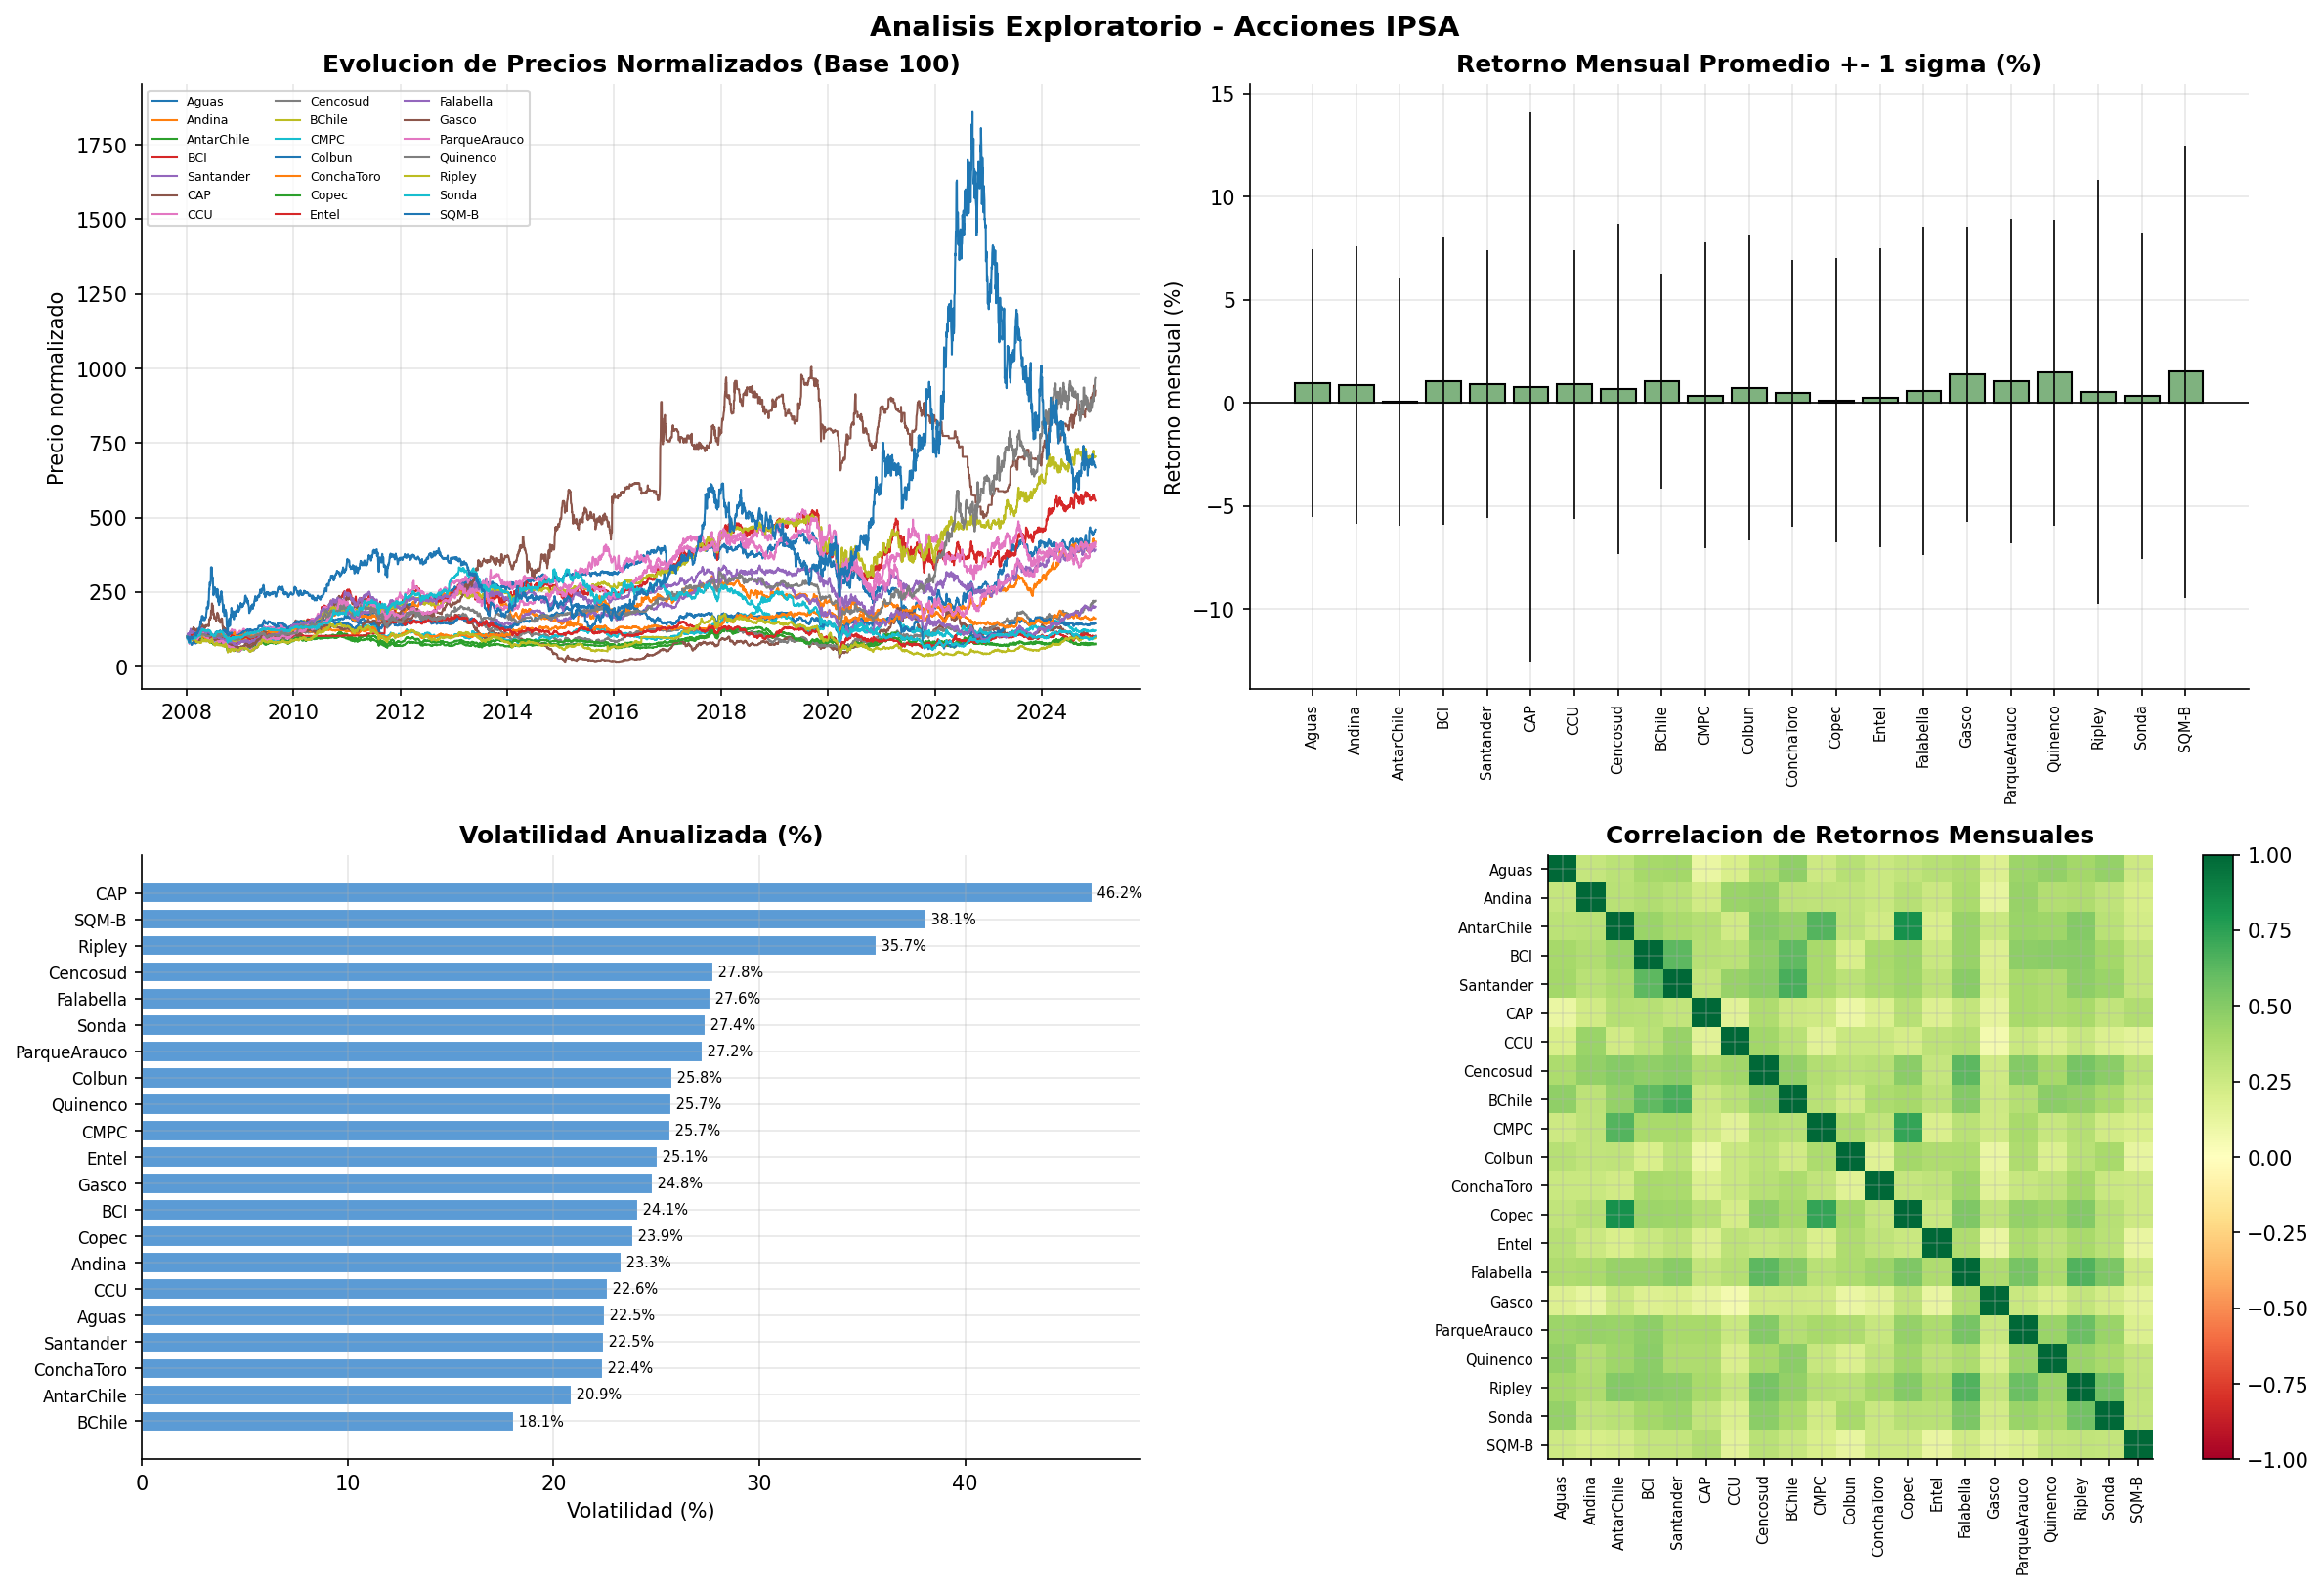
\includegraphics[width=0.92\textwidth]{fig_eda.png}
\caption{Análisis exploratorio del universo de 21 acciones del IPSA (2008--2024).}
\label{fig:eda}
\end{figure}

\paragraph{Desempeño de las estrategias.} El Cuadro~\ref{tab:metricas} muestra el desempeño de las
seis estrategias y la Figura~\ref{fig:backtest} su evolución. En retorno y Sharpe, el ML Ridge
encabeza la tabla (Sharpe $0.296$) y el 1/N queda en el medio ($0.125$). Pero el patrón importante
aparece en las columnas de riesgo: la mínima varianza logra la menor volatilidad ($13.7\%$), muy por
debajo del resto. En el otro extremo, el DFL ---pese a estar diseñado para optimizar el
Sharpe de forma directa--- queda \emph{último} en Sharpe ($0.046$) y con un
\emph{turnover} desproporcionado ($1.10$ frente a $0.045$ del 1/N). Ese exceso de rotación es la
primera señal de un modelo que se sobreajusta a la ventana de entrenamiento.

\begin{table}[H]
\centering
\caption{Métricas de desempeño en el walk-forward (155 meses, 2012--2024).}
\label{tab:metricas}
\begin{tabular}{lrrrrrr}
\toprule
Estrategia & Ret.\ acum. & CAGR & Vol.\ anual & Sharpe & Max DD & Turnover\\
\midrule
1/N (Equal-Weight)     & $109.5\%$ & $5.9\%$ & $15.8\%$ & $0.125$ & $-40.7\%$ & $0.045$\\
Markowitz clásico      & $164.6\%$ & $7.8\%$ & $15.7\%$ & $0.240$ & $-37.9\%$ & $0.280$\\
Markowitz + Ledoit--Wolf & $163.8\%$ & $7.8\%$ & $15.8\%$ & $0.238$ & $-38.9\%$ & $0.275$\\
Mínima Varianza + LW   & $94.6\%$  & $5.3\%$ & $\mathbf{13.7\%}$ & $0.080$ & $-33.6\%$ & $0.141$\\
ML Ridge + LW          & $\mathbf{200.8\%}$ & $\mathbf{8.9\%}$ & $16.6\%$ & $\mathbf{0.296}$ & $-38.0\%$ & $0.677$\\
DFL (MLP directo)      & $78.0\%$  & $4.6\%$ & $16.0\%$ & $0.046$ & $-31.8\%$ & $1.102$\\
\bottomrule
\end{tabular}
\end{table}

\begin{figure}[H]
\centering
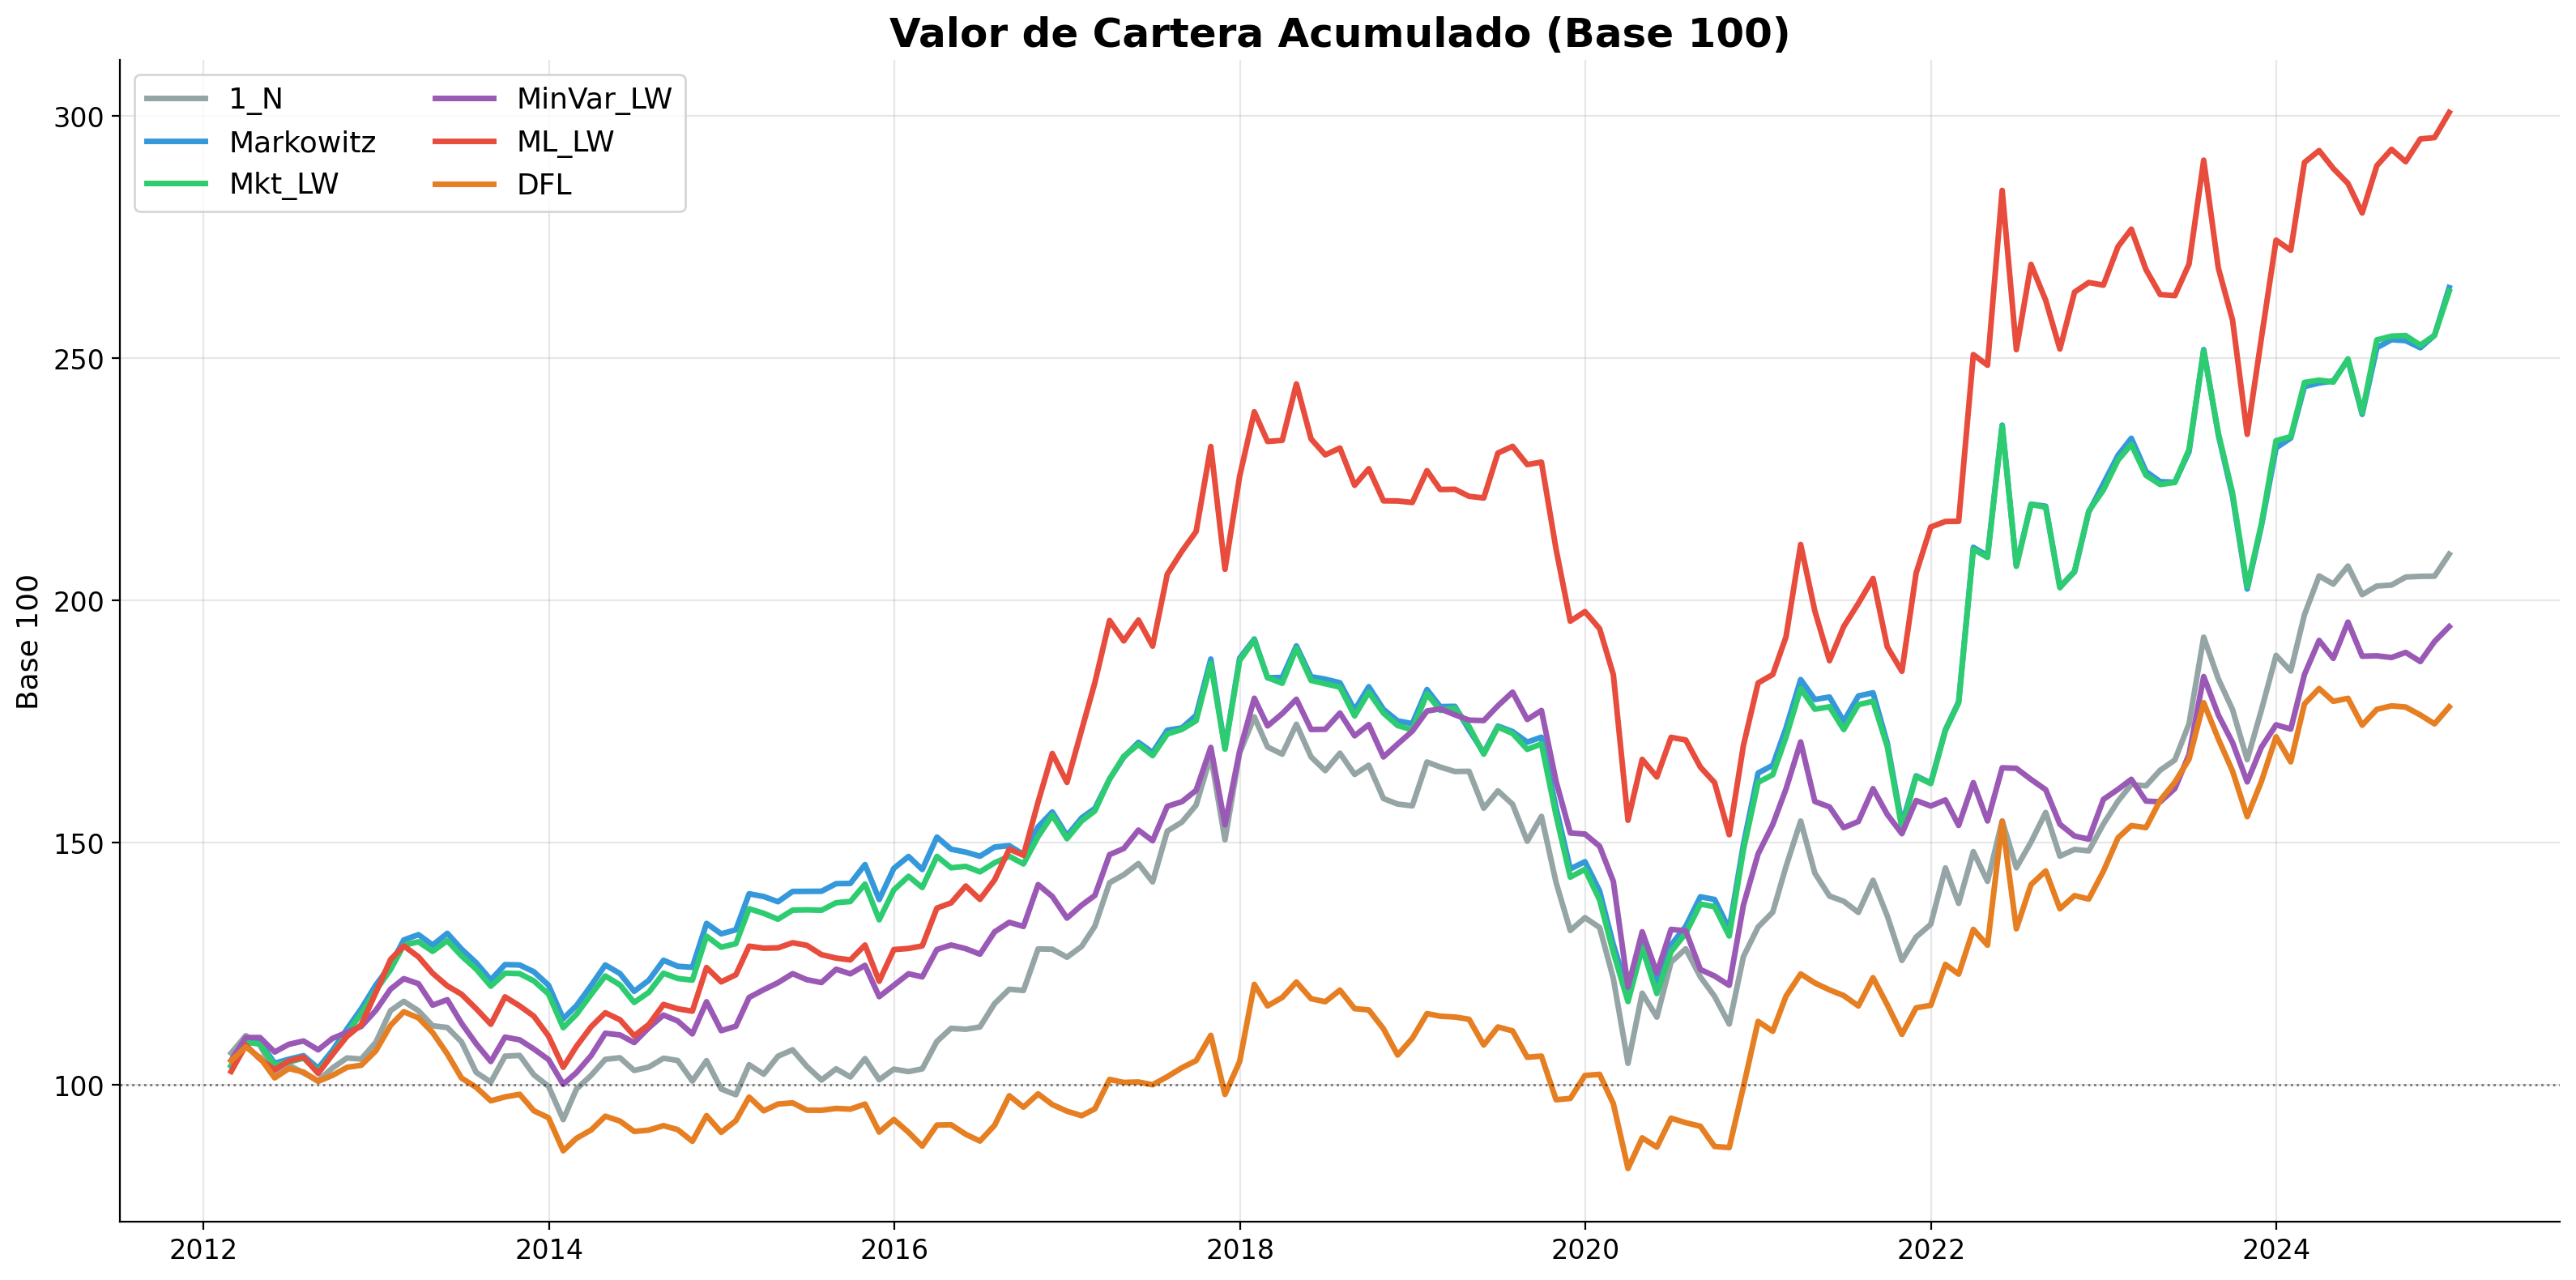
\includegraphics[width=0.95\textwidth]{figs/fig_backtest_cartera.png}
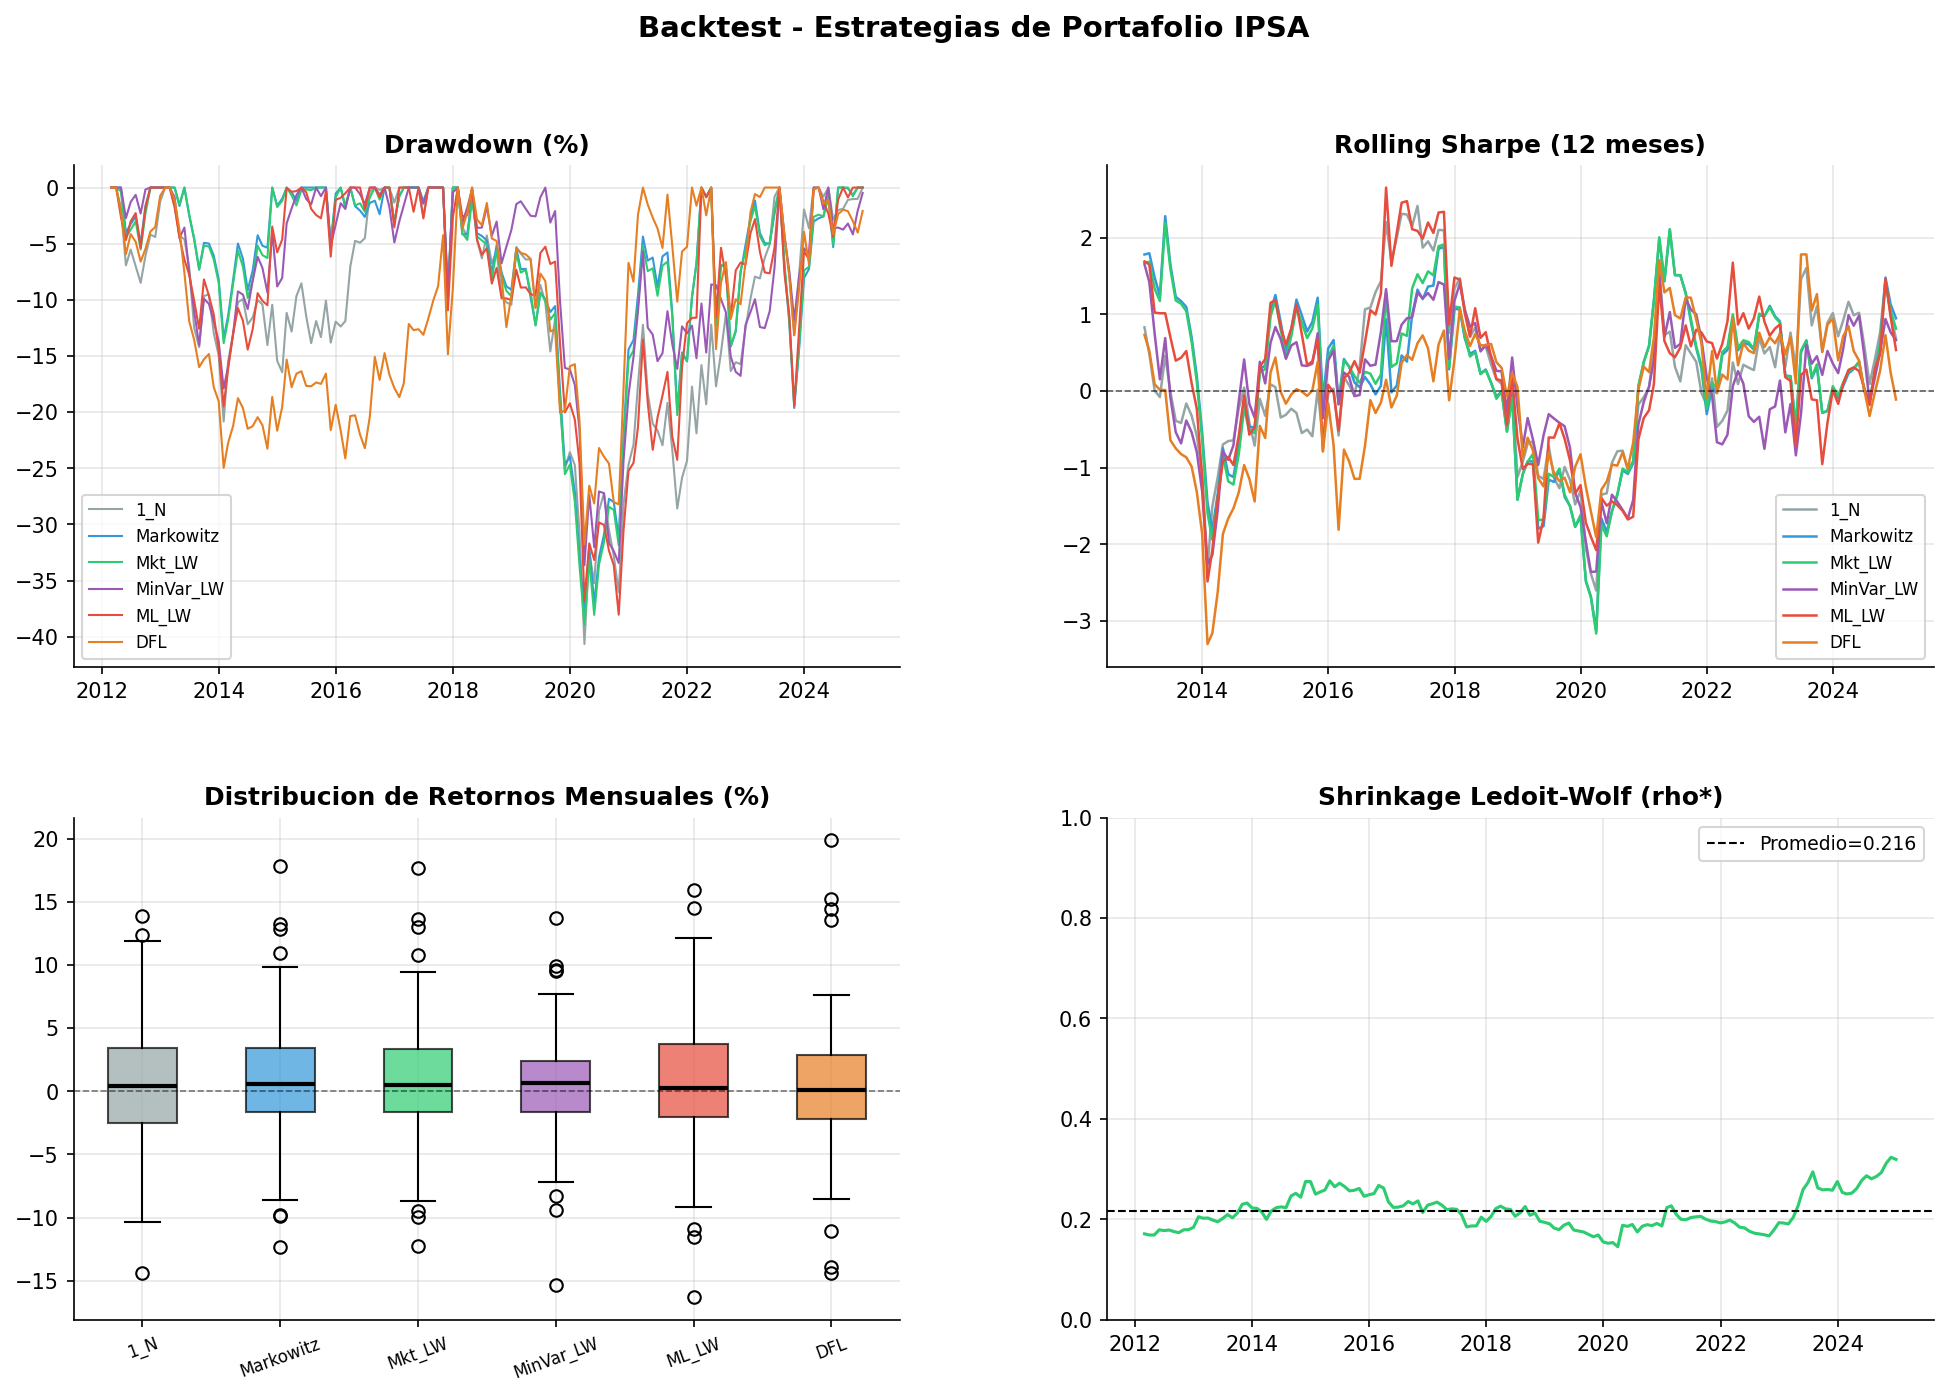
\includegraphics[width=0.95\textwidth]{figs/fig_backtest_panel.png}
\caption{Comparación de las seis estrategias: valor acumulado, \emph{drawdowns}, rolling Sharpe,
distribución de retornos y evolución del \emph{shrinkage} de Ledoit--Wolf.}
\label{fig:backtest}
\end{figure}

\paragraph{El predictor de retornos no tiene señal.} El poder
predictivo se mide con la \Roos: si es positiva, el modelo predice mejor que usar la media histórica;
si es negativa, predice \emph{peor}. La \Roos\ del Ridge es $-0.085$ (con un \emph{Information
Coefficient} $\text{IC}=+0.008$, prácticamente cero): el modelo no aporta información sobre los
retornos futuros. El contraste con su \Roos\ \emph{in-sample} ($+0.097$, positiva) es la firma de que hay sobreajuste: aprende muy bien el pasado y no generaliza nada. El Cuadro~\ref{tab:mse}
y la Figura~\ref{fig:comp} confirman que esto \textbf{no depende del modelo}: ninguno de los cuatro
---lineales o MLP--- logra \Roos\ positiva. Por lo tanto, el aparente buen Sharpe del ML+LW ($0.296$)
no viene de acertarle a los retornos, sino del optimizador y de la covarianza.

\begin{table}[H]
\centering
\caption{Comparación de modelos ML (hiperparámetros por MSE). Sharpe del 1/N $= 0.125$.}
\label{tab:mse}
\begin{tabular}{lrrrrr}
\toprule
Modelo & \Roos & IC & MSE & Sharpe$_{\text{ML}}$ & vs.\ 1/N\\
\midrule
Ridge       & $-0.085$ & $+0.008$ & $0.00661$ & $0.296$ & $+0.171$\\
Lasso       & $-0.037$ & $+0.022$ & $0.00632$ & $0.267$ & $+0.142$\\
Elastic Net & $-0.042$ & $+0.022$ & $0.00634$ & $0.247$ & $+0.122$\\
MLP         & $-0.054$ & $-0.013$ & $0.00642$ & $0.197$ & $+0.072$\\
\bottomrule
\end{tabular}
\end{table}

\begin{figure}[H]
\centering
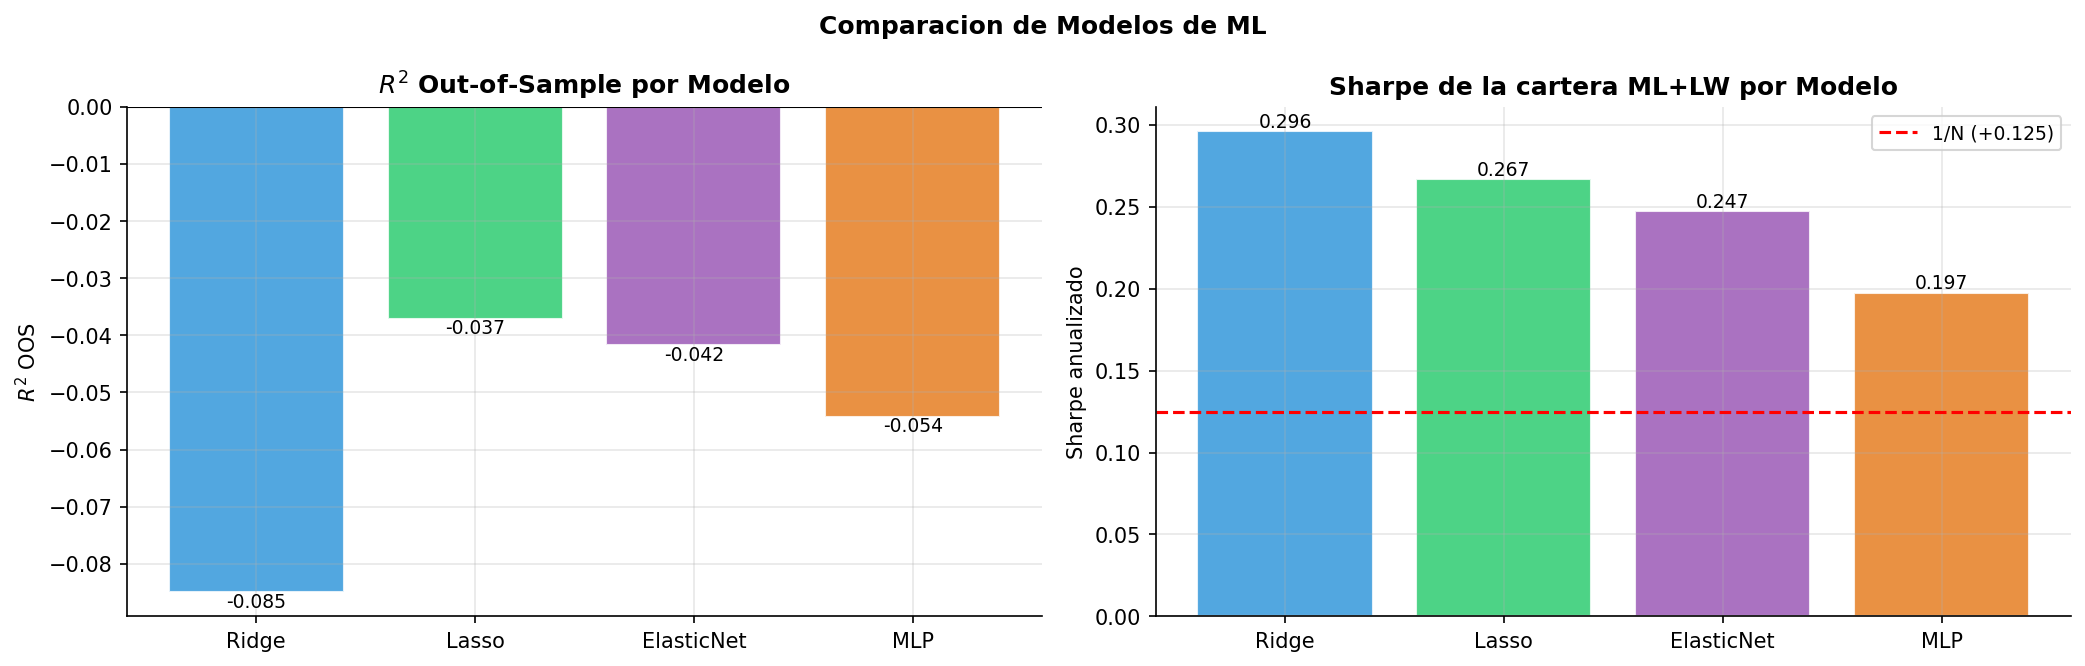
\includegraphics[width=0.85\textwidth]{fig_comparacion_modelos.png}
\caption{Poder predictivo (\Roos) y Sharpe de la cartera ML+LW por modelo. Ningún modelo alcanza
\Roos\ positiva.}
\label{fig:comp}
\end{figure}

\paragraph{Afinar directamente por Sharpe no rescata el resultado.} El Cuadro~\ref{tab:sharpe} repite
el ejercicio, pero eligiendo la regularización por Sharpe en validación interna. La \Roos\ sigue
negativa (de hecho empeora, porque el criterio ya no busca predecir bien) y el Sharpe del mejor modelo
apenas llega a $0.160$. Esto no es contradictorio, ya que al no haber señal, el Sharpe de validación ---calculado
sobre 12 meses--- es esencialmente ruido, y afinar un parámetro para maximizar ruido no mejora nada
fuera de muestra. La evidencia más clara está en \emph{qué} regularización se elige: para el mejor
modelo afinado (Lasso), el \texttt{alpha} no converge a un valor, sino que se reparte a lo largo de
los 155 meses ($\alpha=0.1$ en 79 meses, $\alpha=0.01$ en 38 y $\alpha=0.001$ en 38). Si existiera una
señal estable, la selección convergería a un valor; que no lo haga confirma que no hay nada estable
que optimizar. El DFL replica el patrón: su Sharpe es $0.046$, por debajo del 1/N.

\begin{table}[H]
\centering
\caption{Modelos ML con hiperparámetros elegidos por Sharpe (validación interna, sin fuga).}
\label{tab:sharpe}
\begin{tabular}{lrrrr}
\toprule
Modelo & \Roos & IC & Sharpe$_{\text{ML}}$ & vs.\ 1/N\\
\midrule
Ridge       & $-0.251$ & $-0.006$ & $0.150$ & $+0.025$\\
Lasso       & $-0.113$ & $+0.017$ & $0.160$ & $+0.035$\\
Elastic Net & $-0.106$ & $+0.003$ & $0.044$ & $-0.081$\\
\bottomrule
\end{tabular}
\end{table}

\paragraph{Ninguna diferencia es significativa.} El \emph{bootstrap} por bloques confirma lo anterior
(Cuadro~\ref{tab:boot} y Figura~\ref{fig:boot}). Los intervalos de confianza al
95\% de los seis Sharpe \textbf{incluyen el cero}, así que ninguna estrategia tiene siquiera un Sharpe
distinguible de cero. Y ninguna supera al 1/N de forma significativa: todos los $p \geq 0.23$. El
mejor candidato, el ML+LW, da $p=0.234$; el mejor ML afinado por Sharpe (Lasso), $p=0.831$. Dicho de
otro modo, con este período de datos no podemos afirmar que ninguna estrategia le gane al reparto
ingenuo.

\begin{table}[H]
\centering
\caption{Bootstrap del Sharpe: estimación, intervalo de confianza 95\% y $p$-valor de la diferencia
contra 1/N.}
\label{tab:boot}
\begin{tabular}{lrcr}
\toprule
Estrategia & Sharpe & IC 95\% & $p$ vs.\ 1/N\\
\midrule
1/N (Equal-Weight)     & $0.125$ & $[-0.376,\ +0.581]$ & ---\\
Markowitz clásico      & $0.240$ & $[-0.308,\ +0.738]$ & $0.536$\\
Markowitz + Ledoit--Wolf & $0.238$ & $[-0.310,\ +0.740]$ & $0.512$\\
Mínima Varianza + LW   & $0.080$ & $[-0.453,\ +0.554]$ & $0.626$\\
ML Ridge + LW          & $0.296$ & $[-0.219,\ +0.773]$ & $0.234$\\
DFL (MLP directo)      & $0.046$ & $[-0.470,\ +0.488]$ & $0.604$\\
\bottomrule
\end{tabular}
\end{table}

\begin{figure}[H]
\centering
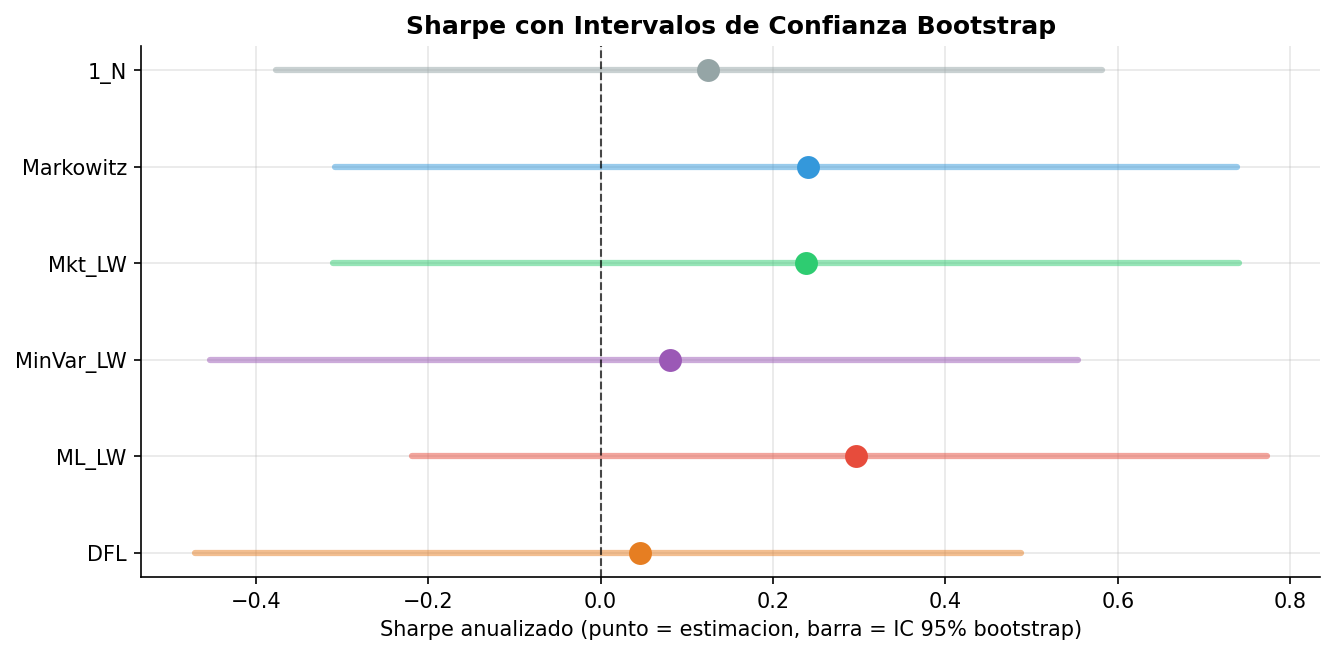
\includegraphics[width=0.72\textwidth]{fig_bootstrap.png}
\caption{Sharpe anualizado con intervalos de confianza bootstrap. Todos los intervalos cruzan el cero
(línea punteada): ninguna estrategia es estadísticamente superior.}
\label{fig:boot}
\end{figure}

\section{Discusión}
El resultado principal es que \textbf{ninguna de las estrategias optimizadas supera al 1/N de manera
estadísticamente distinguible}. Las mejoras de Sharpe son marginales y se evaporan al cuantificar su
incertidumbre: con 155 meses de test, el error de estimación del Sharpe es tan grande que las
diferencias observadas son indistinguibles del azar.

Lejos de ser anómalo, esto reproduce el hallazgo central de DeMiguel, Garlappi y Uppal (2009). Al
comparar 14 modelos de optimización de portafolio contra el reparto ingenuo 1/N en múltiples conjuntos
de datos, esos autores encontraron que ninguno lo superaba de forma consistente fuera de muestra. La
causa es el \textbf{error de estimación de los parámetros} ---sobre todo de los retornos esperados
$\mu$---, que el optimizador de Markowitz amplifica en lugar de corregir. El 1/N, al no estimar nada,
no sufre ese error. Nuestro experimento confirma el mecanismo de forma directa: $\mu$ no es predecible
en esta muestra (ni con la media histórica ni con ningún modelo ML, cuya \Roos\ es negativa en todos
los casos), de modo que optimizar en base a $\mu$ no puede agregar valor.

El caso del DFL es ilustrativo por sí solo. Una arquitectura diseñada para maximizar el Sharpe de
forma directa termina siendo la de peor Sharpe entre las seis ($0.046$) y con el mayor
\emph{turnover}. Es exactamente el sobreajuste que cabía esperar: al maximizar el Sharpe
\emph{in-sample} de una ventana corta, la red persigue patrones que no se repiten fuera de muestra.

La única dimensión donde sí aparece una diferencia consistente ---aunque no en Sharpe--- es el
\textbf{riesgo}. La mínima varianza, que ignora por completo $\mu$, entrega una de las menores volatilidades. Para un inversionista cuyo objetivo es controlar el riesgo, es preferible; no
porque ``gane'' en términos ajustados por riesgo, sino porque obtiene un Sharpe equivalente con caídas
más suaves.

\section{Conclusión}
Construimos y evaluamos, de forma honesta y fuera de muestra, dos familias de modelos ML para asignar
un portafolio del IPSA ---modelos que predicen $\mu$ y un MLP de asignación directa---, con covarianza
robusta, validación sin fuga de información, costos y restricciones de concentración. A pesar de esa
sofisticación, no encontramos evidencia de que superen al 1/N en Sharpe: todas las \Roos\ son
negativas y ninguna estrategia es estadísticamente distinguible del reparto ingenuo. El valor del
trabajo es metodológico: una evaluación walk-forward sin fuga, la medición explícita del poder
predictivo fuera de muestra y un test de significancia que evita confundir ruido con habilidad. El
cierre defendible es que, con los datos y \emph{features} disponibles, ni la predicción de retornos ni
la asignación directa por ML le ganan al 1/N, y la única ventaja real ---en riesgo--- la ofrece una
estrategia que ni siquiera intenta predecir retornos.

\section{Limitaciones}
\label{sec:limitaciones}
\begin{itemize}[nosep,leftmargin=*]
  \item \textbf{Sesgo de supervivencia.} El universo incluye sólo acciones que siguen listadas y
  líquidas hoy, lo que infla levemente todos los resultados.
  \item \textbf{Poder estadístico.} Con 155 meses de test, el error de estimación del Sharpe es grande
  para magnitudes tan pequeñas; los intervalos de confianza son anchos por construcción.
  \item \textbf{Features.} Se limitan a momentum y volatilidad; no se exploran señales fundamentales
  ni macroeconómicas (p.\ ej.\ precio del cobre o USD/CLP).
  \item \textbf{Sobreajuste del DFL.} La red de asignación directa maximiza el Sharpe \emph{in-sample}
  de una ventana corta; pese a la regularización, el criterio es intrínsecamente propenso a
  sobreajustar, como confirma su desempeño.
\end{itemize}


\section{Apéndice: fórmulas de las métricas}
\label{sec:formulas}
Esta sección deja registro de cómo se calculó cada medida y, sobre todo, de cómo interpretarla.
Notación: $r_t$ es el retorno mensual de la cartera en el mes $t$ (ya descontados los costos),
$r_f$ la tasa libre de riesgo mensual, $\overline{x}$ el promedio de una cantidad $x$ sobre los
$T=155$ meses de test y $\hat{\sigma}$ la desviación estándar muestral. El retorno neto de un mes es
el retorno bruto de la cartera menos lo que cuesta rebalancearla:
\[
r_t \;=\; \underbrace{\mathbf{w}_t^{\top}\mathbf{r}_t}_{\text{retorno bruto}}
\;-\; \underbrace{c\textstyle\sum_i |w_{i,t}-w_{i,t}^{-}|}_{\text{costo de mover la cartera}},
\qquad c = 0.1\%,
\]
donde $w_{i,t}^{-}$ es el peso de la acción $i$ justo antes de rebalancear.
 
\subsection*{Métricas de desempeño}
 
\paragraph{Sharpe.} Mide cuánto retorno se obtiene por cada unidad de riesgo. Toma el retorno
promedio por sobre la tasa libre de riesgo y lo divide por su volatilidad:
\[
\text{Sharpe} \;=\; \frac{\overline{r-r_f}}{\hat{\sigma}_{r-r_f}}\;\sqrt{12}.
\]
Cuanto más alto, mejor. El factor $\sqrt{12}$ lo lleva de escala mensual a anual. A grandes rasgos, un
Sharpe de $0.1$ dice que el retorno anual en exceso equivale a una décima de la volatilidad anual.
 
\paragraph{Sortino.} Es un Sharpe que sólo castiga la volatilidad ``mala''. En lugar de la desviación
total usa la \emph{desviación a la baja} $\mathrm{DD}$, que ignora los meses buenos:
\[
\text{Sortino} \;=\; \frac{\overline{r-r_f}}{\mathrm{DD}}\;\sqrt{12},
\qquad
\mathrm{DD} \;=\; \sqrt{\tfrac{1}{T}\sum_{t=1}^{T}\big[\min(r_t-r_f,\,0)\big]^2}.
\]
El $\min(\cdot,0)$ deja pasar sólo los meses en que el retorno cayó bajo $r_f$; los meses positivos
entran como cero. Se divide por el total de meses $T$ (no sólo por los negativos), de modo que la
métrica refleja el \emph{tamaño} de las caídas y no cuántas hubo.
 
\paragraph{Volatilidad anual y CAGR.} La primera es la dispersión de los retornos; la segunda, la
tasa de crecimiento anual compuesta que, aplicada constante, reproduce el resultado final:
\[
\sigma_{\text{anual}} \;=\; \hat{\sigma}_r\,\sqrt{12},
\qquad\qquad
\text{CAGR} \;=\; \Big(\prod_{t=1}^{T}(1+r_t)\Big)^{12/T}-1.
\]
El producto $\prod_t (1+r_t)$ es cuánto crece un peso invertido a lo largo del test; el exponente
$12/T$ convierte ese crecimiento total en un equivalente por año.
 
\paragraph{Máximo \emph{drawdown} y Calmar.} El \emph{drawdown} de un mes es cuánto ha caído la
cartera desde su punto más alto previo; el máximo \emph{drawdown} es la peor de esas caídas. Con
$V_t=\prod_{s\le t}(1+r_s)$ el valor acumulado:
\[
\text{MaxDD} \;=\; \min_{t}\ \frac{V_t-\max_{s\le t}V_s}{\max_{s\le t}V_s},
\qquad\qquad
\text{Calmar} \;=\; \frac{\text{CAGR}}{|\text{MaxDD}|}.
\]
$\max_{s\le t}V_s$ es el máximo histórico hasta $t$, y la fracción mide qué tan por
debajo del máximo se está. El Calmar relaciona el crecimiento anual con esa peor caída.
 
\paragraph{Turnover.} Cuánto se reordena la cartera en cada rebalanceo, sumando los cambios de peso
de todas las acciones y promediando sobre los $R$ rebalanceos:
\[
\text{Turnover} \;=\; \frac{1}{R}\sum_{t\,\in\,\text{rebal}}\ \sum_i \big|w_{i,t}-w_{i,t}^{-}\big|.
\]
Un valor alto implica mucha rotación (y más costos): el $1.10$ del DFL frente a $0.045$ del 1/N indica
que el DFL rehace casi por completo la cartera cada mes.
 
\subsection*{Cuán bien predice el modelo}
 
\paragraph{$R^2$ fuera de muestra e IC.} Sobre todos los pares (acción, mes) del período de test, con
$r$ el retorno realizado y $\hat{\mu}$ la predicción:
\[
R^2_{\text{oos}} \;=\; 1 - \frac{\sum (r-\hat{\mu})^2}{\sum (r-\bar{r})^2},
\qquad\qquad
\text{IC} \;=\; \operatorname{corr}(\hat{\mu},\,r).
\]
El $R^2_{\text{oos}}$ compara dos errores: el del modelo (numerador) contra el de ``predecir siempre
el promedio'' $\bar{r}$ (denominador). Si el modelo le gana al promedio, la fracción es menor que $1$
y $R^2_{\text{oos}}>0$; si es peor, la fracción supera $1$ y $R^2_{\text{oos}}<0$ ---justo nuestro
caso, que indica ausencia de señal. El $R^2_{\text{in}}$ es la misma fórmula, pero medida dentro de la
ventana de entrenamiento (promediada sobre acciones y ventanas); que sea positivo mientras el de fuera
de muestra es negativo es la señal clásica de sobreajuste. El IC (\emph{Information Coefficient}) es la
correlación de Pearson entre lo predicho y lo realizado: un valor cercano a $0$ significa que la
predicción no se relaciona con lo que efectivamente pasó.
 
\subsection*{Optimización de cartera}
 
Los pesos salen de un optimizador que usa la covarianza $\Sigma$ estabilizada con \emph{shrinkage} de
Ledoit--Wolf,
\[
\hat{\Sigma}_{\text{LW}} \;=\; (1-\delta)\,\mathbf{S} \;+\; \delta\,\mathbf{F},
\]
una mezcla entre la covarianza muestral $\mathbf{S}$ (precisa pero ruidosa con pocos datos) y un
objetivo estructurado y estable $\mathbf{F}$; la intensidad $\delta\in[0,1]$ se elige de forma
automática. Con esa $\Sigma$, cada estrategia resuelve uno de dos problemas:
\[
\begin{aligned}
\text{máx.\ Sharpe:}&\quad \max_{\mathbf{w}}\ \frac{\mathbf{w}^{\top}(\boldsymbol{\mu}-r_f\mathbf{1})}
{\sqrt{\mathbf{w}^{\top}\Sigma\,\mathbf{w}}},\\[4pt]
\text{mín.\ varianza:}&\quad \min_{\mathbf{w}}\ \mathbf{w}^{\top}\Sigma\,\mathbf{w},
\end{aligned}
\]
ambos con $\sum_i w_i=1$ (todo el capital invertido) y $0\le w_i\le 0.20$ (sin ventas en corto y con
tope de $20\%$ por acción). En el máximo Sharpe, el numerador es el retorno esperado de la cartera y
el denominador su volatilidad. La mínima varianza minimiza sólo esa volatilidad y ni siquiera mira
$\boldsymbol{\mu}$, por lo que es inmune al error de estimar los retornos esperados.



\paragraph{Markowitz (clásico y +Ledoit--Wolf).} No hay modelo predictivo: el retorno esperado de cada
acción es simplemente su promedio histórico dentro de la ventana,
$\hat{\mu}_i = \overline{r}_{i,\,\text{ventana}}$, y la covarianza es la muestral $\mathbf{S}$ (clásico)
o su versión con \emph{shrinkage} $\hat{\Sigma}_{\text{LW}}$ (+Ledoit--Wolf). Con eso resuelve el
problema de máximo Sharpe ya visto:
\[
\max_{\mathbf{w}}\ \frac{\mathbf{w}^{\top}(\hat{\boldsymbol{\mu}}-r_f\mathbf{1})}
{\sqrt{\mathbf{w}^{\top}\Sigma\,\mathbf{w}}},
\qquad \text{s.a. } \sum_i w_i = 1,\ \ 0\le w_i\le 0.20.
\]
 
\paragraph{Ridge.} Para cada acción $i$ ajusta coeficientes $\boldsymbol{\beta}_i$ que predicen su
retorno a partir de las \emph{features}, penalizando la magnitud \emph{cuadrática} de los
coeficientes:
\[
\hat{\boldsymbol{\beta}}_i^{\text{Ridge}}
\;=\; \arg\min_{\boldsymbol{\beta}}\ \sum_{t}\big(r_{i,t}-\mathbf{x}_{i,t-1}^{\top}\boldsymbol{\beta}\big)^2
\;+\; \alpha\sum_j \beta_j^2 .
\]
La penalización $L_2$ ($\alpha\sum_j\beta_j^2$) achica todos los coeficientes hacia cero de forma
proporcional, sin anular ninguno. Mientras más grande $\alpha$, más se ``aplana'' el modelo hacia
predecir la media: la validación cruzada elige un $\alpha$ alto porque no hay
señal que valga la pena capturar.


\paragraph{ML Ridge + LW.} Es el ensamble de las dos piezas
anteriores: la predicción de Ridge entra como $\hat{\boldsymbol{\mu}}$ al optimizador de máximo
Sharpe, usando la covarianza con \emph{shrinkage} de Ledoit--Wolf. Para cada mes $t$ del test:
\begin{align*}
    \hat{\mu}_{i} &= \mathbf{x}_{i,t-1}^{\top}\hat{\boldsymbol{\beta}}_i^{\text{Ridge}}
\quad\text{para cada acción } i,\\
\mathbf{w}_t &= \arg\max_{\mathbf{w}}\ \frac{\mathbf{w}^{\top}(\hat{\boldsymbol{\mu}}-r_f\mathbf{1})}
{\sqrt{\mathbf{w}^{\top}\hat{\Sigma}_{\text{LW}}\,\mathbf{w}}},
\qquad \text{s.a. } \sum_i w_i = 1,\ \ 0\le w_i\le 0.20.
\end{align*}
Es decir, $\hat{\boldsymbol{\mu}}$ ya no es el promedio histórico (como en Markowitz), sino la
predicción de Ridge; la covarianza $\hat{\Sigma}_{\text{LW}}$ es la misma que usa
``Markowitz + Ledoit--Wolf''.

 
\paragraph{Lasso.} Misma idea que Ridge, cambiando la penalización cuadrática por una en valor
absoluto:
\[
\hat{\boldsymbol{\beta}}_i^{\text{Lasso}}
\;=\; \arg\min_{\boldsymbol{\beta}}\ \sum_{t}\big(r_{i,t}-\mathbf{x}_{i,t-1}^{\top}\boldsymbol{\beta}\big)^2
\;+\; \alpha\sum_j |\beta_j| .
\]
La penalización $L_1$ puede llevar coeficientes exactamente a \textbf{cero}, no sólo achicarlos: hace
selección automática de \emph{features}, mientras que Ridge las mantiene todas (aunque pequeñas).
 
\paragraph{Elastic Net.} Combina ambas penalizaciones con un parámetro de mezcla $\rho\in[0,1]$:
\[
\hat{\boldsymbol{\beta}}_i^{\text{EN}}
\;=\; \arg\min_{\boldsymbol{\beta}}\ \sum_{t}\big(r_{i,t}-\mathbf{x}_{i,t-1}^{\top}\boldsymbol{\beta}\big)^2
\;+\; \alpha\Big[\rho\sum_j |\beta_j| \;+\; \tfrac{1-\rho}{2}\sum_j \beta_j^2\Big].
\]
Con $\rho=1$ es Lasso puro; con $\rho=0$, Ridge puro. Es útil cuando hay \emph{features} muy
correlacionadas entre sí --como ocurre con nuestras 9 \emph{features}, varias de las cuales miden
variantes de lo mismo--: Lasso puro tiende a elegir una del grupo casi al azar y descartar el resto,
mientras Elastic Net las reparte de forma más estable.
 
En los tres modelos anteriores, $\alpha$ (y $\rho$ para Elastic Net) se elige por validación cruzada
\emph{dentro} de la ventana de entrenamiento, sin tocar el mes a predecir. El retorno esperado
resultante es $\hat{\mu}_i = \mathbf{x}_{i,t-1}^{\top}\hat{\boldsymbol{\beta}}_i$, y ese vector
$\hat{\boldsymbol{\mu}}$ es el que recibe el optimizador de máximo Sharpe (con covarianza
Ledoit--Wolf) para obtener los pesos finales.
 
\paragraph{El modelo MLP de asignación directa (\emph{decision-focused learning}).}
Aquí no hay paso intermedio de predecir $\mu$: una red $f_\theta$ toma las \emph{features} de todas
las acciones y entrega directamente los pesos de la cartera,
\[
\mathbf{w}_t \;=\; \text{softmax}\big(f_\theta(\mathbf{X}_{t-1})\big),
\]
(o una capa de salida equivalente que garantice $\sum_i w_i=1$, $w_i\ge 0$), entrenada minimizando el
negativo del Sharpe de la cartera resultante sobre la ventana de entrenamiento:
\[
\theta^{*} \;=\; \arg\min_{\theta}\ -\,\text{Sharpe}\big(\{\mathbf{w}_t^{\top}\mathbf{r}_t\}_{t\,\in\,\text{train}}\big).
\]
La diferencia de fondo con Ridge (u otros modelos que predicen $\mu$) más Markowitz: ahí se optimizan
dos objetivos en dos pasos separados --primero minimizar el error de predicción, después maximizar el
Sharpe dado $\hat{\boldsymbol{\mu}}$--; acá se optimiza un único objetivo de punta a punta (de ahí el
nombre \emph{decision-focused}: la red aprende directamente para la decisión final, no para un paso
intermedio).

\paragraph{Evidencia de la regularización elegida.} Esto se puede verificar directamente en el
$\alpha$ que elige \texttt{GridSearchCV} en los $155\times21=3255$ ajustes del walk-forward
(Cuadro~5). En Ridge, Lasso y Elastic Net la moda cae de forma sistemática en el extremo más
regularizado, y en Lasso/EN es
un valor interior, lo que descarta que sea un artefacto de la grilla. El MLP no
replica el patrón: su $\alpha$ se reparte casi parejo entre ambos extremos ($38.7\%$ vs.\ $39.8\%$),
más consistente con ruido de estimación que con una preferencia estable.

\begin{table}[h]
\centering
\caption{$\alpha$ elegido por validación cruzada (MSE), sobre 3255 ajustes.}
\begin{tabular}{lccc}
\toprule
Modelo & $\alpha$ modal & \% en la moda & ¿Tope de la grilla? \\
\midrule
Ridge       & $10\,000$ & $56.0\%$ & Sí \\
Lasso       & $0.1$     & $82.2\%$ & No \\
Elastic Net & $0.1$     & $86.6\%$ & No \\
MLP         & $100$     & $39.8\%$ & Ambiguo \\
\bottomrule
\end{tabular}
\end{table}

 
\subsection*{Test de significancia (bootstrap por bloques)}
 
Para saber si una diferencia de Sharpe es real o suerte del período, remuestreamos la historia muchas
veces y observamos cuánto varía el resultado. En cada una de las $5000$ réplicas se arma una serie
``alternativa'' pegando bloques contiguos de $L=6$ meses tomados al azar y se recalcula el Sharpe. Los mismos bloques se
aplican a todas las estrategias (remuestreo pareado), de modo que la comparación es justa. El intervalo
de confianza al $95\%$ son los percentiles $2.5$ y $97.5$ de esos $5000$ Sharpe. Para comparar una
estrategia contra el 1/N miramos, en cada réplica, la diferencia
$d^{*}=\text{Sharpe}^{*}_{\text{estr}}-\text{Sharpe}^{*}_{1/N}$, y el $p$-valor a dos colas es
\[
p \;=\; 2\,\min\big\{\Pr(d^{*}\le 0),\ \Pr(d^{*}\ge 0)\big\}.
\]
Un $p$ grande, como los que obtuvimos, significa que la diferencia observada cabe cómodamente dentro
de lo que produce el puro azar: no es distinguible de cero.


\paragraph{Referencia.}
DeMiguel, V., Garlappi, L., \& Uppal, R. (2009). \emph{Optimal Versus Naive Diversification: How
Inefficient Is the 1/N Portfolio Strategy?} Review of Financial Studies, 22(5), 1915--1953.

\end{document}